\input{../preamble.tex}

\SetDate[16/04/2026]
\reversemarginpar
\setlength{\marginparsep}{.5cm}

\begin{document}
\pagestyle{fancy}
\fancyhead[L]{Première}
\fancyhead[C]{\textbf{Évaluation — Dérivation}}
\fancyhead[R]{\today}

\null\vspace{-30pt}
Consignes particulières : 
\begin{itemize}[label=$\bullet$]
	\item 
	La calculatrice est {interdite}.
	\item
	L'évaluation fait \pageref{lastpage} pages. La somme des points est \total{points}.
\end{itemize}

\marginpar{[pts]}
\hrule

%\subsection*{Automatismes}



\exe{4,difficulty=0}{
	Considérons la fonction $f$ donnée graphiquement ci-dessous.
	\begin{enumerate}
		\item 
		Quel est le signe de $f(-3)$ ?
		\item 
		Quel est le signe de $f'(-3)$ ? Justifier.
		\item 
		Donner approximativement la valeur de $f'(-1,7)$. Justifier.
		\item
		La tangente à $\C_f$ en $x=-1$ a pour équation $y = 5,75x + 4,34$.
		En déduire la valeur de $f'(1)$.
	\end{enumerate}

	\begin{center}
	\begin{tikzpicture}[>=stealth, scale=1]
	\begin{axis}[xmin=-4, xmax=1, ymin=-4, ymax=4, axis x line=middle, axis y line=middle, axis line style=-, grid=both, xtick distance = 1, ytick distance = 2, minor y tick num = 1, clip=false]
		\addplot[BLUE_E, very thick, domain=-4:1, samples=100] {-6.5 + 10*e^(-x^2) -x + .3*x^2}  node[right] {$\C_{f}$};
		\addplot[RED_E, <->, thick, domain=-1.5:-.5, samples=2, xshift=.5pt] {5.75759*x+4.23638}  node[pos=0, right] {$y = 5,75x + 4,34$};
	\end{axis}
	\end{tikzpicture}
	\end{center}

}{exe:tangente-graphique}{
%	\begin{enumerate}
%		\item 
%		En se plaçant en $x=2$, on lit $f(2) \approx -1,5$ et donc que
%		$f(2)$ est négatif.
%		\item 
%		En $x=2$, la courbe descend et $f$ est décroissante.
%		D'après le cours, $f'(2) < 0$.
%		\item 
%		En $x=3$, la tangente à la courbe est horizontale, son coefficient directeur est donc nul.
%		On en déduit que $f'(3) \approx 0$.
%		
%		Une autre façon d'obtenir le résultat est de la façon suivante :
%		autour de $x=3$, la fonction $f$ passe de décroissante à croissante.
%		Le signe de $f'(x)$ est donc négatif puis positif, et passe donc nécessairement par 0.
%		\item
%		$f'(1)$ est, par définition, le coefficient directeur de la tangente à $\C_f$ en $x=1$.
%		Cette tangente a pour équation $y=8,3-4,4x = -4,4 \times x + 8,3 = ax+b$, avec $a=-4,4$ et $b=8,3$.
%		Seul $a=-4,4$, le coefficient directeur, nous intéresse ici :
%			\[ f'(1) = -4,4. \]
%	\end{enumerate}
}

\exe{3,difficulty=0}{
	La courbe représentative d'un fonction $f$ est donnée ci-dessous.
	Compléter son tableau de signes.

	\begin{multicols}{2}
	\begin{tikzpicture}[>=stealth, scale=1]
	\begin{axis}[xmin=-4, xmax=1, ymin=-4, ymax=4, axis x line=middle, axis y line=middle, axis line style=-, grid=both, xtick distance = 1, ytick distance = 2, minor y tick num = 1, clip=false]
		\addplot[GREEN_E, very thick, domain=-4:1, samples=100] {-(-6.5 + 10*e^(-x^2) -x + .3*x^2)}  node[right] {$\C_{f}$};
	\end{axis}
	\end{tikzpicture}
	\hfill
	\vfill
	\begin{tikzpicture}
		\tkzTabInit
		 %[lgt=3,espcl=1.5]
	       		{$x$ / 1 , Signe de $f(x)$ / 2}
	       		{,,}
	\end{tikzpicture}
	\vfill\null
	\end{multicols}
}{exe:lecture-graphique}{
%	Lorsque $\C_f$ est au-dessus de l'axe des abscisses, $f(x)$ est positif.
%	Lorsque $\C_f$ est en-dessous, $f(x)$ est négatif.
%	
%	On obtient donc environ le tableau suivant.
%	Les $x$ importants auxquels $f(x)$ change de signe sont ceux pour lesquels $f(x) = 0$ : les intersections entre $\C_f$ et l'axe des abscisses.
%	\begin{center}
%	\begin{tikzpicture}
%		\tkzTabInit
%		 %[lgt=3,espcl=1.5]
%	       		{$x$ / 1 , Signe de $f(x)$ / 2}
%	       		{0, {0,6}, 2,3}
%		\tkzTabLine
%			{z,+,z,-,z,+}
%	\end{tikzpicture}
%	\end{center}
}




%\subsection*{Exercice}


\exe{3}{
	Donner la fonction dérivée de chaque fonction suivante.
	\begin{multicols}{2}
	\begin{enumerate}
		\item $f(x) = 2x^3 + x^2 + 2x + 1$
		\item $g(x) = 31 - 3x - 6x^2 + x^3$
	\end{enumerate}
	\end{multicols}
	
	Donnée :
	\begin{center}
	\begin{tabular}{|c|c|c|c|c|}\hline
		Monôme & 1 & $x$ & $x^2$ & $x^3$ \\ \hline
		Dérivée & {0} & {1} & {$2x$} & {$3x^2$} \\ \hline
	\end{tabular}
	\end{center}
}{exe:derivation}{
	On utilise d'un part que $(f+g)' = f'+g'$ et que $(c\times f)' = c\times f'$ pour $f, g$ deux fonctions et $c$ un nombre.
	D'autre part, le tableau suivant permet de dériver les monômes de degré inférieurs à 3.
	\begin{center}
	\begin{tabular}{|c|c|c|c|c|}\hline
		Monôme & 1 & $x$ & $x^2$ & $x^3$ \\ \hline
		Dérivée & {0} & {1} & {$2x$} & {$3x^2$} \\ \hline
	\end{tabular}
	\end{center}
	Moyen mnémotechnique : $(x^n)' = n\times x^{n-1}$.
	La puissance sort en multiple et est diminuée de 1.
%	\begin{enumerate}
%		\item 
%			\begin{align*}
%				f'(x) &= (x^3 + 2x^2 + 6x + 10)' \\
%						&= (x^3)' + (2x^2)' + (6x)' + (10)' \\
%						&= (x^3)' + 2(x^2)' + 6(x)' + 10(1)' \\
%						&= 3x^2 + 2\times2x + 6\times1 + 10\times 0 \\
%						&= 3x^2 + 4x + 6
%			\end{align*}
%		\item 
%			\begin{align*}
%				g'(x) &= (-x^2 + 7x - 1)' \\
%						&= -(x^2)' + 7(x)' - 1' \\
%						&= -2x + 7
%			\end{align*}
%	\end{enumerate}
}

\exe{4}{
	Développer et réduire chaque expression suivante.
	\begin{multicols}{3}
	\begin{enumerate}
		\item $f(x) = (x+4)(x-1)$
		\item $g(x) = (2x+1)(x+3)$
		\item $h(x) = 3(x+1)(x-1)$
	\end{enumerate}
	\end{multicols}
}{exe:dev-red}{
	On utilise la double distributivité classique
		\[ (a+b)(c+d) = ac+ad+bc+bd. \]
%	\begin{enumerate}
%		\item 
%			\begin{align*}
%				f(x) &= (x+1)(x+2) \\
%						&= x^2 + x + 2x + 2 \\
%						&= x^2 + 3x + 2
%			\end{align*}
%		\item
%			\begin{align*}
%				g(x) &= (2x-3)(x+2) \\
%						&= 2x^2 + 4x - 3x - 6 \\
%						&= 2x^2 + x - 6
%			\end{align*}
%		\item 
%			\begin{align*}
%				h(x) &= 3(x+1)(x-4) \\
%						&= 3\bigl[(x+1)(x-4)\bigr] \\
%						&= 3\bigl[x^2 + x - 4x - 4\bigr] \\
%						&= 3\bigl[x^2 - 3x - 4\bigr] \\
%						&= 3x^2 - 9x - 12
%			\end{align*}
%	\end{enumerate}
}

\exe{6,difficulty=1}{
	Nous étudions une fonction $f$ pour des antécédents $x$ situés entre $-3$ et $2$.
	
	Nous disposons des informations suivantes sur $f$.
	\begin{multicols}{2}
	\begin{itemize}
		\item
		Sa dérivée est 
			$ f'(x) = (2x+3)(x-1). $
		\item
		L'image de $-3$ est $f(-3) \approx -4,6$
		\item
		L'image de $-1,5$ est $f(-1,5) \approx 3,2$
		\item
		L'image de 1 est $f(1) = -2$
		\item
		L'image de 2 est $f(2) \approx 1,2$
	\end{itemize}
	\end{multicols}
	\begin{enumerate}
		\item Remplir le tableau de signes et de variations de la figure \ref{fig:var-signe}.
		\item Compléter les variations avec les images connues de $f$.
		\item En déduire le maximum et le minimum de $f$ sur le domaine d'étude.
		\item Utiliser le tableau de variations pour esquisser $\C_f$ dans le repère figure \ref{fig:Cf}.
	\end{enumerate}
}{exe:variations-d3}{
	Pour étudier le signe de $ax+b$, on trouve le $x$ pour lequel la fonction s'annule en posant $ax+b=0 \iff x = \frac{-b}a$.
	
	Ensuite, soit en testant des valeurs de $x$, soit en regardant le signe du coefficient directeur $a$ de la fonction, on décide des signes de part et d'autre du zéro.
	
	Ici, pour $2x+3$, nous trouvons
		\begin{align*}
			2x+3 &= 0 \\
			2x &= -3 \\
			x &= \frac{-3}2 \\
			x &= -1,5
		\end{align*}
	De plus, avant $-1,5$ la fonction $2x+5$ est négative.
	En $x=-3$ par exemple, $2x+5 = 2\times(-3) + 5 = -6+5 = -1 < 0$.
	Enfin, après $-1,5$ la fonction $2x+5$ est positive.
	En $x=2$ par exemple, $2x+5 = 2\times2+5 = 9 > 0$.
	
	On fait idem avec la fonction $x-1$ puis $f'(x)$, le produit des deux, pour obtenir le tableau suivant.
	\begin{center}
	\begin{tikzpicture}
		\tkzTabInit
		 %[lgt=3,espcl=1.5]
	       		{$x$ / 1 , Signe de $2x+3$ / 1, Signe de $x-1$ / 1, Signe de $f'(x)$ / 1, Variation de $f(x)$ / 2}
	       		{$-3$,{-1,5},1,2}
		\tkzTabLine
			{,-,z,,,+,}
		\tkzTabLine
			{,,-,,z,+,}
		\tkzTabLine
			{,+,z,-,z,+,}
		\tkzTabVar
			{-/{-4,6},+/{3,2},-/{-2},+/{1,2}}
	\end{tikzpicture}
	\end{center}
	
	La courbe représentative de la fonction $f$ ressemble à ceci.
	
	Le maximum de $f$ est $f(-1,5) \approx 3,2$.
	Le minimum de $f$ est $f(-3) \approx -4,6$.
	Ce sont respectivement la plus grande et la plus petite valeur du tableau de variations.
	
	\begin{center}
	\begin{tikzpicture}[scale=1.2]
	\begin{axis}[
		xmin = -3, xmax=2,
		ymin=-5, ymax=5,
		axis x line=middle, 
		axis y line=middle, 
		axis line style=-,
		grid = both, % xlabel={$x$}, ylabel={$f(x)$},
		minor tick num = 1,
	%xtick = {0, 0.2, ..., 1.4},
	%ytick = {-1, -0.5, 0, .5, 1.5},
	]
	\addplot[domain=-3:2, BLUE_E, thick, samples=100] {2*x^3/3 + x^2/2 - 3*x-1/6} node[right]{$\C_f$};
	\end{axis}
	\end{tikzpicture}
	\end{center}

}


\begin{figure}[h]
	\centering	
	\begin{tikzpicture}
		\tkzTabInit
		 %[lgt=3,espcl=1.5]
	       		{$x$ / 1 , Signe de $2x+3$ / 1, Signe de $x-1$ / 1, Signe de $f'(x)$ / 1, Variation de $f(x)$ / 2}
	       		{$-3$,,,,2}
	\end{tikzpicture}
	\caption{Tableau de variations de $f$ et de signes de $f'$.}
	\label{fig:var-signe}
\end{figure}

\begin{figure}[h]
	\centering
	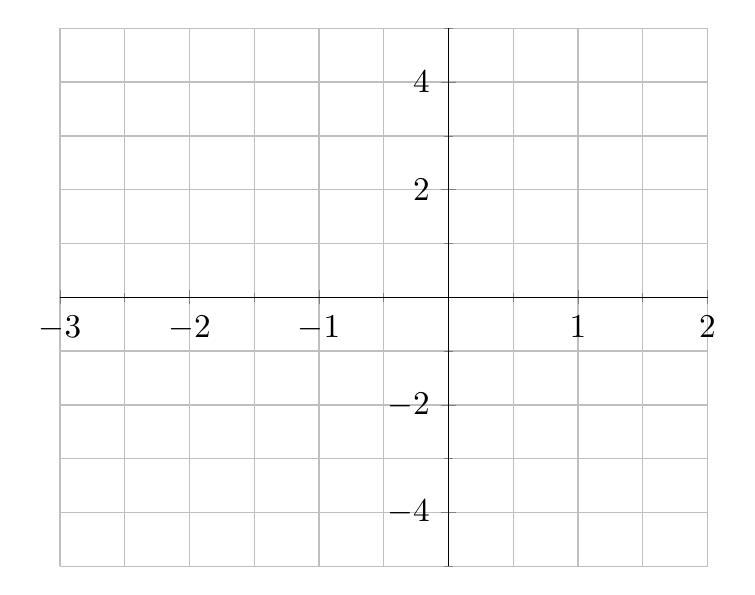
\begin{tikzpicture}[scale=1.2]
	\begin{axis}[
		xmin = -3, xmax=2,
		ymin=-5, ymax=5,
		axis x line=middle, 
		axis y line=middle, 
		axis line style=-,
		grid = both, % xlabel={$x$}, ylabel={$f(x)$},
		minor tick num = 1,
	%xtick = {0, 0.2, ..., 1.4},
	%ytick = {-1, -0.5, 0, .5, 1.5},
	]
	\addplot[domain=-3:2, transparent, thick, samples=100] {2*x^3/3 + x^2/2 - 3*x-1/6} node[right]{$\C_f$};
	\end{axis}
	\end{tikzpicture}
	\caption{Graphe approximatif de $\C_f$.}
	\label{fig:Cf}
\end{figure}


%%%%%%%%%%%%

\label{lastpage}
\newpage
\fancyhead[C]{\textbf{Solutions}}
\shipoutAnswer

\end{document}
